\section{Limits}

\subsection{Delta-Epsilon Definition on R}

The limit of $f$ as $x$ approaches $a$ is $L$ if given a positive real number
$\epsilon$, there exists a corresponding $\delta$ so that numbers selected with distance from $a$
less than $\delta$ and $>0$ it is guaranteed that outputs under $f$ are within distance $\epsilon$ from $L$.

Formal definition:

$\lim_{x\to a}f(x)=L$ if $\forall \epsilon >0$, $\exists\delta > 0$ such that $0< |x-a| < \delta \implies |f(x)-L|<\epsilon$

\subsection{Definition of Limit on R2}

If $f:\R^2\to \R$ and $P_0=(x_0,y_0)$, then $\lim _{(x, y) \rightarrow\left(x_{0}, y_{0}\right)} f(x, y)=L$ 
if given any small positive number $\epsilon$, $\delta>0$ is guaranteed so when there is a point $C\neq P_0$ within circle of radius $\delta$ about $P_0$, $f(x,y)$ lies within $\epsilon$ of $L$.

Formally: 

\[\lim _{(x, y) \rightarrow\left(x_{0}, y_{0}\right)} f(x, y)=\lim _{\vec{x} \rightarrow P_{0}} f(x, y)=L \text { if } \forall \varepsilon>0 \;\exists \delta>0\]

such that

\[0<\sqrt{\left(x-x_{0}\right)^{2}+\left(y-y_{0}\right)^{2}}<\delta \Longrightarrow|f(x, y)-L|<\varepsilon\]

\subsection{Continuous Functions}

\begin{itemize}
    \item Polynomials: $f(x,y)=x^2y+xy^2$
    \item Exponentials: $f(x,y)=e^{xy}$
    \item Trigonometric: $f(x,y)=\sin(x+y)$
    \item Compositions of any continuous functions: $f(x,y)=\cos(e^{x^2y-xy^2})$
    \item Sums, differences, products of continuous functions: $f(x, y)=x^{2} y-x y^{2}+e^{x y} \sin (x y)$
    \item Quotients of continuous functions (domain of quotient does not include zeros of denominator): $f(x, y)=\frac{x^{2 y}-x y^{2}}{\sin (x y)}$
\end{itemize}

\subsection{Computational Techniques}

Can use continuity to find limit (plug in point). Can also use conjugate multiplication to simplify and compute. Cancelling terms works because a limit approaches a value instead of equaling it.
Can also squeeze a function between 2 continuous ones to find limit.

Let $\lim _{(x, y) \rightarrow(0,0)} \frac{x^{2}}{\sqrt{x^{2}+y^{2}}}$ exist.
Know that $0\leq \lim _{(x, y) \rightarrow(0,0)} \frac{x^{2}}{\sqrt{x^{2}+y^{2}}}$.
Because $y^2>0$, $\frac{x^{2}}{\sqrt{x^{2}+y^{2}}} \leq \frac{x^{2}+y^{2}}{\sqrt{x^{2}+y^{2}}}$.
Thus, $\lim _{(x, y) \rightarrow(0,0)} 0 \leq \lim _{(x, y) \rightarrow(0,0)} \frac{x^{2}}{\sqrt{x^{2}+y^{2}}} \leq \lim _{(x, y) \rightarrow(0,0)}\left(x^{2}+y^{2}\right)^{1 / 2}$
so the limit is 0.

Other strategies: If a term $k(x,y)\geq 0\;\forall\; (x,y)\in \R^2$, then can simply perform $\pm 1$ to denominator for squeeze theorem proofs.

\subsection{Common inequalities and proofs}

\begin{itemize}
    \item AM-GM inequality: $\frac{x+y}{2}\geq \sqrt{xy}\implies (x-y)^2\geq 0$
    \item Triangle inequality: $|x+y|\leq |x|+|y|$ and $|x-y|\geq |x|-|y|$
    \item $|e^x-1|\leq |x|e^{|x|}$
\end{itemize}

Proof that $\frac{\sin x}{x}=1$:

\begin{center}
    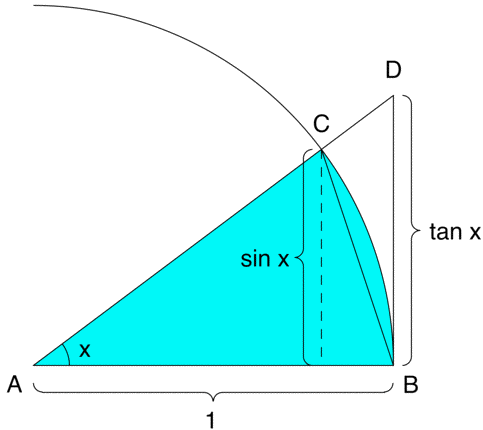
\includegraphics[scale=0.4]{Screen Shot 2021-04-21 at 10.59.12 AM.png}
\end{center}

It is evident that:
\begin{gather}
    \frac{1}{2}\sin x\leq \frac{1}{2}x\leq \frac{1}{2}\tan x\\
    \sin x\leq x \leq \tan x\\
    1\leq \frac{x}{\sin x}\leq \frac{1}{\cos x}\\
    1\geq \frac{\sin x}{x}\geq \cos x
\end{gather}

Applying the squeeze theorem to 4:

\begin{gather*}
    \lim_{x\to 0}1\geq \lim_{x\to 0}\frac{\sin x}{x}\geq \lim_{x\to 0} \cos x\\
    1\geq \frac{\sin x}{x}\geq 1
\end{gather*}

Thus, $\lim_{x\to 0}\frac{\sin x}{x}=1$.

\section{Derivatives}

\subsection{Limit Definition}

A function $f:\R^m \to \R^n$ is differentiable at $P_0$ if there is a linear transformation from $n\times m$ matrix $Df(P_0)$ satisfying

\[\lim_{\vec{x}\to P_0}\frac{\big\vert \big\vert f \big( \vec{x} \big)-\big(f(P_0)+\mathrm{D}f(P_0)(\vec{x}-P_0) \big) \big\vert \big\vert}{\vert \vert \vec{x}-P_0 \vert \vert}=0\]

If the function is differentiable at this point, then $Df(P_0)$ is the derivative of $f$ at $P_0$. Called Jacobian matrix of $f$ at $P_0$.

Can adapt this to single-variable calculus:

\[\displaystyle \lim_{x\to a} \frac{\vert f(x)-\big(f(a)+(m_a)(x-a)\big) \vert}{\vert x-a \vert}=0\]

Simplifying and reconfiguring to limit definition of a derivative:

\begin{align*}
    \lim_{x\to a} \frac{\vert f(x)-\big(f(a)+(m_a)(x-a)\big) \vert}{\vert x-a \vert}&=0\\
    \lim_{x\to a}\left\vert \frac{f(x)-\big(f(a)+(m_a)(x-a)\big)}{x-a} \right\vert&=0\\
    \left \vert \lim_{x\to a} \frac{f(x)-\big(f(a)+(m_a)(x-a)\big)}{x-a} \right \vert&=0\\
    \lim_{x\to a} \frac{f(x)-\big(f(a)+(m_a)(x-a)\big)}{x-a}&=0 \, \mbox{since}\, \vert 0 \vert=0\\ 
    \lim_{x\to a} \left( \frac{f(x)-f(a)}{x-a}-m_a\right)&=0\\
    \lim_{x\to a}\frac{f(x)-f(a)}{x-a}&=m_a
\end{align*}

Equivalent to the case of a $1\times 1$ matrix $Df(P_0)$ where the single entry is $f'(a)$.
Also $m_a=f'(a)\implies f(x)=f(a)+f'(a)(x-a)$ is the linear approximation. 

As $x$-values approach $a$, $f(x)-(f(a)+f'(a)(x-a))$ approaches 0 faster. Thus, $\frac{f(x)-\big(f(a)+f'(a)(x-a)\big)}{x-a}$ approaches 0.

\subsection{Multivariable Application}

Approximating plane of some $f:\R^2\to \R$ is $L_{P_0}(x,y)=f(a,b)+f_x(a,b)(x-a)+f_y(a,b)(y-b)$, i.e. the plane spanned by
$\langle 1,0,f_x(a,b)\rangle$ and $\langle 0,1,f_y(a,b)\rangle$ passing through $(a,b,f(a,b))$.

Is identical to $\begin{bmatrix}f_x(P_0)&f_y(P_0)\end{bmatrix}\begin{bmatrix}x-a\\y-b\end{bmatrix}$. The matrix is the matrix of partial derivatives.

Such a function is differentiable if:

\[\displaystyle \lim_{(x,y)\to(a,b)}\frac{f(x,y)-\left(f(a,b)+\Big(\begin{matrix} f_x(a,b)&f_y(a,b) \end{matrix} \Big)\left(\begin{matrix}x-a\\y-b\\ \end{matrix} \right) \right)}{\sqrt{(x-a)^2+(y-b)^2}}=0\]

Numerator is linear approximation and denominator is distance to point $(a,b)$. Thus:

\[\boxed{f(x,y) \mbox{ is differentiable at the point }P_0\mbox{ if}\displaystyle \lim_{(x,y)\to P_0}\frac{|f(x,y)-L_{P_0}(x,y)|}{||(x,y)-P_0||}=0}\]

Geometrically, if a circle about $P_0$ is drawn and radius is collapsed, distance between $f$ and approximating plane will become 0 much faster, so fraction becomes 0.

If there is a radius $\delta > 0$ on the disk of radius $\delta$ centered at $P_0$, $f_x(x,y)$ and $f_y(x,y)$ are continuous at every point on the disk, then $f(x,y)$ is continious at every point on the disk.
Differentiability can not be established by the existence of partial derivatives at a point, it is sufficient to demonstrate continuous partials
at a point.

If a function $f:\R^m\to \R^n$ exists, then it is made up of $n$ component functions on $\R^m$. The Jacobian matrix is as follows:

\[Df\left( x_1,\ldots x_m\right) =\begin{bmatrix} \nabla f_{1}\left(x_1,\ldots x_m\right) \\ \vdots \\ \nabla f_{n}\left(x_1,\ldots x_m\right) \end{bmatrix}\]

The number of rows $n$ depends on components (codomain) of the output space whereas the domain determines columns ($m$). Thus, linear approximation to a function $f:\R^m\to \R^n$ at $P_0$ is

\[L_{P_0}(\vec{x})=f(P_0)+\Big(\mbox{matrix of partial derivatives at}\,P_0\Big)(\vec{x}-P_0)\]

In parametric equations (paths), let $\vec{c}(t)=\big(x(t), y(t), z(t) \big)$ have continuous partials.
Thus, the matrix of partials $D\vec c(t)=\begin{bmatrix}x'(t)\\y'(t)\\z'(t)\end{bmatrix}$. Is the vertical velocity vector.
If the approximation $L_{t_0}(t)$ is found, it yields:

\begin{align*}
    L_{t_0}(t)&=\vec c(t_0)+
    \left(
    \begin{matrix}
    x'(t_0)\\
    y'(t_0)\\
    z'(t_0)\\
    \end{matrix}
    \right)
    (t-t_0)\\
    &=\vec{c} (t_0)+(t-t_0)\vec c\,'(t_0)
\end{align*}

Also, note that matrix of partials for a scalar valued function $f:\R^n\to \R$ is simply the gradient; there is 1 row and $n$ columns in the gradient vector.